\documentclass[conference]{IEEEtran}
\usepackage{cite}
\usepackage{amsmath,amssymb}
\usepackage{graphicx}
\usepackage{booktabs}
\usepackage{array}
\usepackage{url}
\usepackage{xcolor}
\usepackage[font=small]{caption}
\usepackage{tikz}
\usetikzlibrary{arrows.meta,positioning,shapes.geometric,calc,backgrounds,fit}

\definecolor{ink}{RGB}{26,26,26}
\definecolor{accent}{RGB}{18,78,120}
\definecolor{steel}{RGB}{82,103,122}
\definecolor{deepred}{RGB}{140,46,38}
\definecolor{deepgreen}{RGB}{30,94,46}
\definecolor{soft}{RGB}{236,239,242}

\begin{document}

\title{Go2 Reinforcement Learning Locomotion\\and Sim-to-Real Transfer}

\author{\IEEEauthorblockN{Richard Albert King Mechoda}
\IEEEauthorblockA{M.Sc. Robotics Engineering, DIBRIS, University of Genoa, Italy\\
Student ID: 8525970 \quad\textbar\quad Cognitive Architectures for Robotics (COGAR)\\
Assignment 13 (E4): RL-Based Locomotion Training and Sim-to-Real Deployment (Simulation and Real Robot)}}

\maketitle

\noindent\textbf{\textit{Abstract.}}\;
We develop, train, validate and deploy a reinforcement-learning locomotion controller for the
Unitree Go2 quadruped. The policy is trained \emph{entirely in simulation} (NVIDIA Isaac Lab,
PPO via RSL-RL, 16{,}384 parallel robots, ${\approx}2\times10^{9}$ steps, 1\,h\,40\,min on one
RTX~PRO~6000) and transferred \emph{zero-shot} to the physical robot through the Unitree SDK and
a ROS\,2 Humble interface. The best flat-terrain policy reaches a 99.7\% episode survival rate
(0.33\% falls), a final return of ${\approx}31.2$, and a 0.22~m/s velocity-tracking error in
simulation, and walks on the real Go2 EDU with no real-world fine-tuning, both from a tethered
laptop and from the onboard Jetson Orin~NX. A rough-terrain policy with a height-scan
observation is trained over stairs and uneven blocks and validated in simulation; its hardware
deployment is pending. We compare two policy configurations to isolate the decisive sim-to-real
factor, an asymmetric actor-critic, and we analyse the sim-to-real gap, its failure cases and
its limitations. Following the COGAR course, we read the system through the Sense-Reasoning/Plan-Act
loop: the learned policy is a \emph{reactive behaviour} (a sensory-to-motor mapping), the
deployment state machine is a \emph{fixed-priority behaviour coordinator} whose safety reflexes
\emph{suppress} the walking behaviour, and several modules instantiate the course's software
design patterns. A short demonstration video is available online.\footnote{Demonstration (Isaac
Lab training to real deployment): \url{https://drive.google.com/file/d/1e1jpoKKcbISyVp17HyGn1CQgQ9hJk3pM/view?usp=sharing}}

\vspace{4pt}
\noindent\textbf{\textit{Index Terms.}}\;
quadruped locomotion, reinforcement learning, sim-to-real transfer, domain randomization,
reactive architectures, behaviour-based robotics.

\section{Research Problem}
\label{sec:problem}

Hand-designing a controller that makes a legged robot walk is difficult, and training one
directly on the physical robot is worse: it is slow, costly and damaging, because learning
requires thousands of falls. The now-standard alternative, used by the leading legged-robotics
groups, is to \emph{learn the controller in simulation}, where thousands of robots can be stepped
in parallel on one GPU~\cite{rudin2022}, and then transfer the result to the real robot. The
central difficulty is the \textbf{sim-to-real gap}: a policy that is excellent in a physics
simulator can fail on hardware, because the simulator is not the world. Friction, actuator
latency, motor-gain errors, mass and contact dynamics all differ, and some quantities the
simulator provides for free, such as the body's linear velocity, cannot be measured on the
robot.

This project addresses that problem for the Unitree Go2 quadruped and, as the COGAR assignment
requires, frames it within \emph{Cognitive Architectures for Robotics}. The objectives, taken
from the assignment brief, are to: set up the Go2 in Isaac Lab and configure the PPO/RSL-RL
pipeline; train flat-terrain walking, trotting and velocity tracking; apply domain randomization
(friction, mass, motor strength, terrain perturbations, observation noise, action delay);
validate in Isaac Sim under perturbations; compare at least two policy configurations; evaluate
velocity-tracking error, falls, orientation stability, cost of transport and disturbance
robustness; export to ONNX/TorchScript and deploy on the real Go2 through the Unitree SDK and
ROS\,2 Humble; run real experiments and compare to simulation; and analyse the sim-to-real gap,
its limitations and possible improvements. Section~\ref{sec:cog} adds the cognitive-architecture
reading the course asks for.

\section{State of the Art}
\label{sec:sota}

Methods that close the sim-to-real gap for learned legged locomotion can be organised by
\emph{where} they attack it (Table~\ref{tab:sota}). The \emph{simulator-fidelity} family reduces
the gap at its source: Tan et al.~\cite{tan2018} transfer Minitaur gaits using accurate actuator
and latency models, and Hwangbo et al.~\cite{hwangbo2019} learn the ANYmal actuator dynamics from
real data. \emph{Domain randomization}, introduced for perception by Tobin et al.~\cite{tobin2017}
and extended to dynamics by Peng et al.~\cite{peng2018}, trains over a distribution of physics so
that reality becomes one more sample. \emph{Privileged learning} changes what the learner
observes: the asymmetric actor-critic of Pinto et al.~\cite{pinto2018} gives the critic full
simulator state while the actor sees only deployable observations, and teacher-student
distillation~\cite{lee2020,miki2022} compresses a privileged teacher into a proprioceptive
student. Finally, massively parallel simulators~\cite{rudin2022} make wide randomization
affordable. This project combines all four families; its distinctive choices, an asymmetric
actor-critic and aggressive actuator-realism randomization, are detailed in
Sections~\ref{sec:method} and~\ref{sec:results}.

\begin{table}[t]
\caption{Four families of sim-to-real approaches for learned legged locomotion.}
\label{tab:sota}
\centering
\footnotesize
\begin{tabular}{p{1.9cm} p{3.3cm} p{2.0cm}}
\toprule
\textbf{Family} & \textbf{Idea / representative works} & \textbf{Main limitation} \\
\midrule
Simulator fidelity / system ID & measured latency, learned actuator nets
(Tan~\cite{tan2018}, Hwangbo~\cite{hwangbo2019}) & per-robot effort; models age \\
\addlinespace
Domain randomization & train over a physics distribution
(Tobin~\cite{tobin2017}, Peng~\cite{peng2018}) & range choice is ad hoc \\
\addlinespace
Privileged learning / adaptation & privileged critic or teacher
(Pinto~\cite{pinto2018}, Lee~\cite{lee2020}, Miki~\cite{miki2022}) & added training complexity \\
\addlinespace
Massive parallel simulation & cheap GPU experience
(Rudin~\cite{rudin2022}) & compute, not design \\
\bottomrule
\end{tabular}
\end{table}

\section{Research Formulation}
\label{sec:method}

\subsection{Hypotheses}
We state three hypotheses before the experiments. \textbf{H1:} in simulation the gap is invisible,
so well-tuned policies all look excellent and a simulation-only evaluation is insufficient.
\textbf{H2:} on hardware, a policy that depends on a quantity the robot cannot measure, the base
linear velocity, drifts, because zeroing that input at deployment puts the policy out of
distribution; an \emph{asymmetric} design that confines the privileged input to the critic walks
straight. \textbf{H3:} heavier action-smoothness penalties and actuator-latency randomization
remove the motor chatter seen on hardware.

\subsection{Learning formulation}
We use Proximal Policy Optimization (PPO)~\cite{schulman2017}, which maximises the expected
discounted return $J(\pi_\theta)=\mathbb{E}_{\tau\sim\pi_\theta}[\sum_t\gamma^t r_t]$ through the
clipped surrogate objective
$L=\mathbb{E}_t[\min(\rho_t\hat{A}_t,\mathrm{clip}(\rho_t,1{-}\epsilon,1{+}\epsilon)\hat{A}_t)]$,
with probability ratio $\rho_t$, $\epsilon=0.2$, advantages from GAE ($\gamma=0.99$,
$\lambda=0.95$), and a KL-adaptive learning rate (target KL 0.01). Actor and critic are separate
MLPs $\to256\to256\to128\to$ with ELU activations, about 100k parameters each, small enough for
50~Hz inference on the onboard computer.

\subsection{Observation, action and control}
The \textbf{actor} observes only what the real robot can measure (Table~\ref{tab:obs}): body
angular velocity and projected gravity from the IMU, joint positions and velocities from the
encoders, the velocity command, and the previous action. Projected gravity replaces raw
orientation as a singularity-free, yaw-invariant ``which way is down.'' The \textbf{critic}
additionally receives the privileged base linear velocity (Section~\ref{sec:cog}). The policy
outputs twelve joint-position offsets from a nominal stance,
$q_{\mathrm{target}}=q_{\mathrm{default}}+0.25\,a$, tracked by a 500~Hz PD loop ($K_p{=}40$,
$K_d{=}1.0$ at deployment). Inference runs at 50~Hz, physics at 200~Hz (decimation 4).

\begin{table}[t]
\caption{Actor observation (45 dims, asymmetric configuration).}
\label{tab:obs}
\centering
\footnotesize
\begin{tabular}{l c l}
\toprule
\textbf{Component} & \textbf{Dim} & \textbf{Source} \\
\midrule
Base angular velocity & 3 & IMU gyroscope \\
Projected gravity & 3 & IMU quaternion \\
Velocity command $(v_x,v_y,\omega_z)$ & 3 & operator / planner \\
Joint positions (rel.\ to stance) & 12 & encoders \\
Joint velocities & 12 & encoders \\
Last action & 12 & internal memory \\
\midrule
\textbf{Total} & \textbf{45} & \\
\bottomrule
\end{tabular}
\end{table}

\subsection{Reward and emergent gait}
The reward is a weighted sum of twelve terms (Table~\ref{tab:reward}). No footstep pattern is
prescribed; the trot gait \emph{emerges} from optimising ``track the command, stay upright, lift
the feet, do not waste energy.''

\begin{table}[t]
\caption{Reward terms (final flat configuration).}
\label{tab:reward}
\centering
\footnotesize
\begin{tabular}{l r | l r}
\toprule
\textbf{Positive} & \textbf{w} & \textbf{Negative} & \textbf{w} \\
\midrule
lin.\ vel.\ tracking & $+1.5$ & flat orientation & $-2.5$ \\
ang.\ vel.\ tracking & $+0.75$ & vertical velocity & $-2.0$ \\
foot air time & $+0.5$ & action rate & $-0.25$ \\
& & undesired contacts & $-1.0$ \\
& & feet slide & $-0.25$ \\
& & joint deviation & $-0.1$ \\
& & torques / accel.\ / ang.xy & small \\
\bottomrule
\end{tabular}
\end{table}

\subsection{Domain randomization}
Every episode perturbs the physics (Table~\ref{tab:dr}): mass, centre of mass, friction,
restitution, external forces and pushes, \emph{actuator gains $\pm20\%$}, joint friction and
armature, and \emph{actuator latency 0-20~ms} via Isaac Lab's \texttt{DelayedPDActuator}. Twenty
percent of robots receive a zero command (stand-still training), so the policy also learns to
hold station. The real robot becomes one variant in this distribution.

\begin{table}[t]
\caption{Domain randomization ranges (per episode).}
\label{tab:dr}
\centering
\footnotesize
\begin{tabular}{l l}
\toprule
\textbf{Parameter} & \textbf{Range} \\
\midrule
Body mass & $-2$ to $+4$~kg \\
Centre of mass & $\pm5$~cm (xy), $\pm2$~cm (z) \\
Friction (static / dynamic) & $0.4$-$1.4$ / $0.3$-$1.0$ \\
Actuator gains $K_p,K_d$ & $\pm20\%$ \\
Actuator latency & $0$-$20$~ms (\texttt{DelayedPDActuator}) \\
Joint friction / armature & randomised \\
External force / push & $\pm3$~N / $\pm0.5$~m/s every 10-15~s \\
Stand-still training & 20\% of robots, zero command \\
\bottomrule
\end{tabular}
\end{table}

\subsection{Two configurations and the flat/rough policies}
To satisfy the comparison requirement we train two configurations that differ only in the
observation architecture and actuator-realism randomization. \textbf{Config~A (V2)} is
\emph{symmetric}: a 48-dim actor that includes the base linear velocity. \textbf{Config~B (V3)}
is \emph{asymmetric}: a 45-dim actor (base velocity given only to the critic), plus the delayed
actuator, $\pm20\%$ gain randomization, joint-friction randomization, stand-still training, and a
$5\times$ heavier action-rate penalty. Network, PPO hyper-parameters, parallel environments and
budget are identical. Separately, two terrains are trained: a \textbf{flat} policy (45-dim) and a
\textbf{rough} policy that adds a 187-dim height scan and is trained over stairs and uneven blocks
in all directions (Fig.~\ref{fig:terrain}, right).

\begin{figure*}[t]
\centering
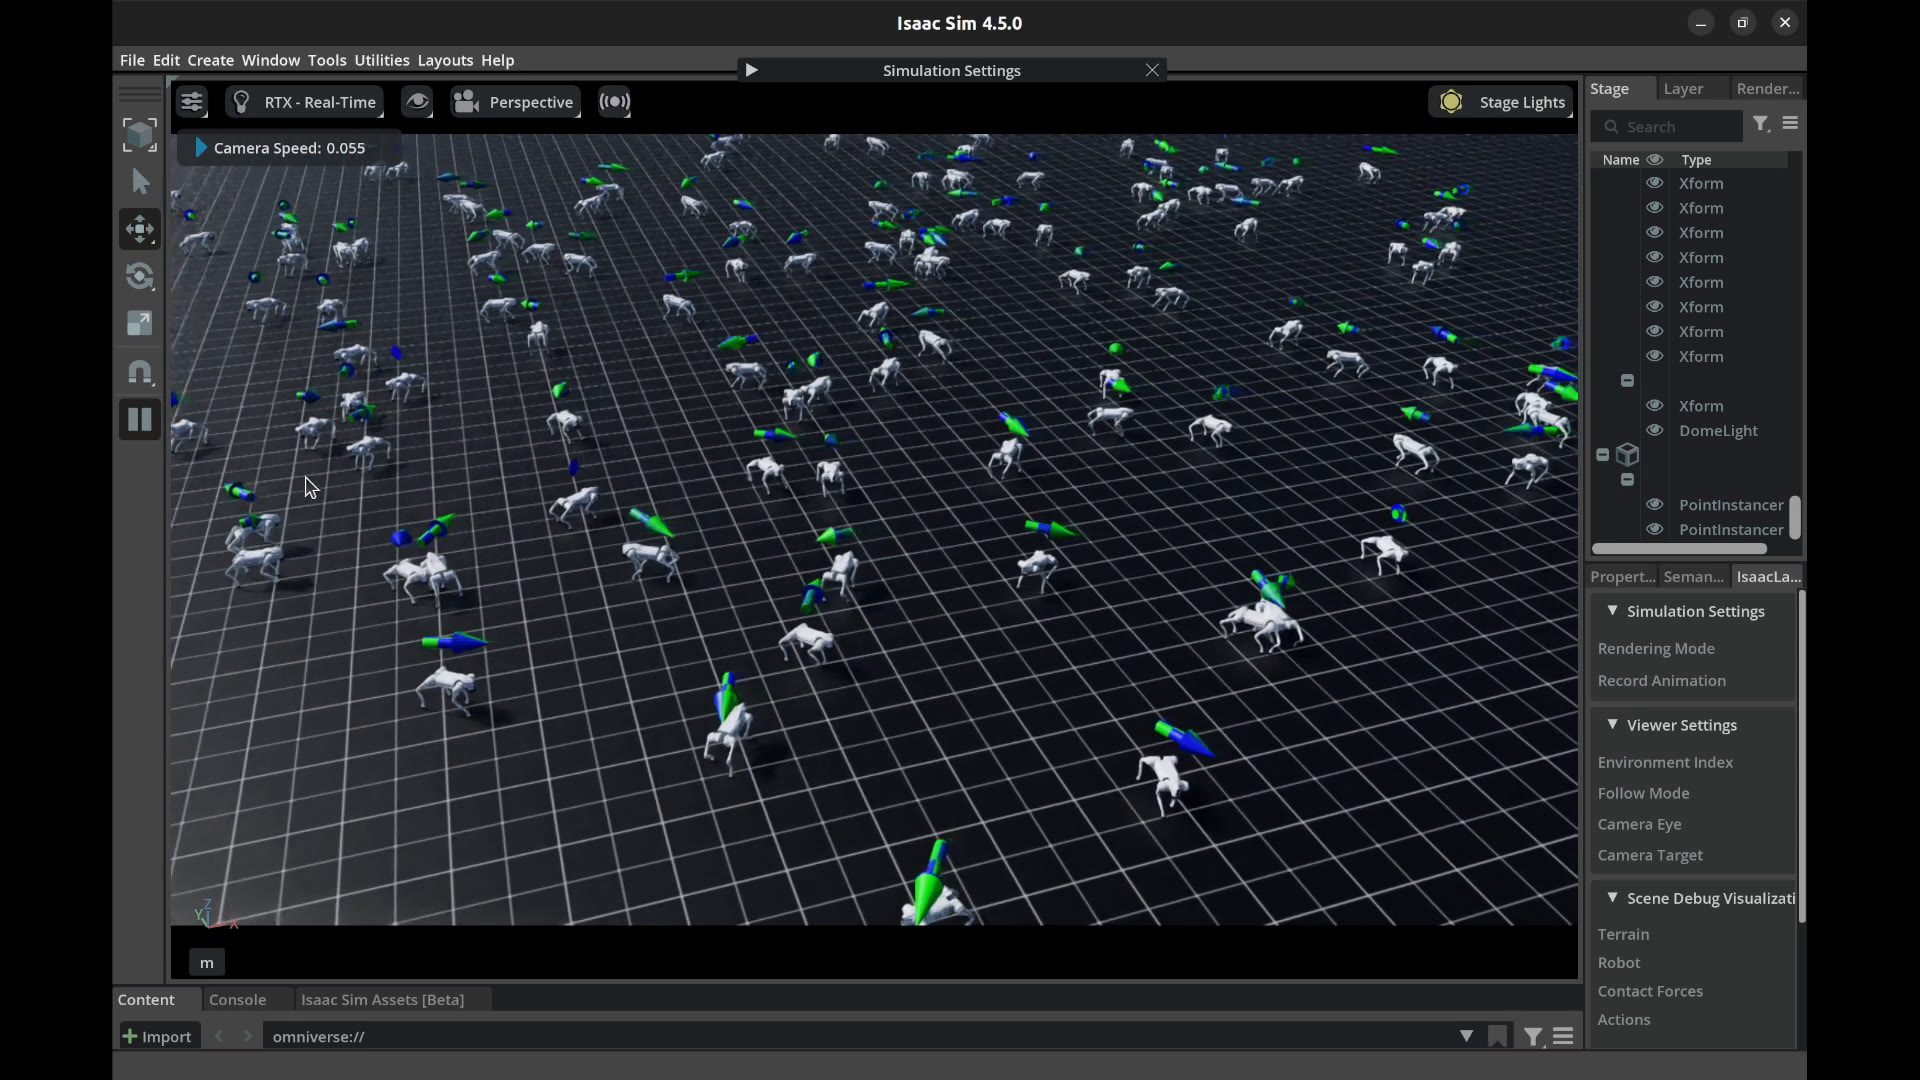
\includegraphics[width=0.485\textwidth]{figures/sim_flat.jpg}\hfill
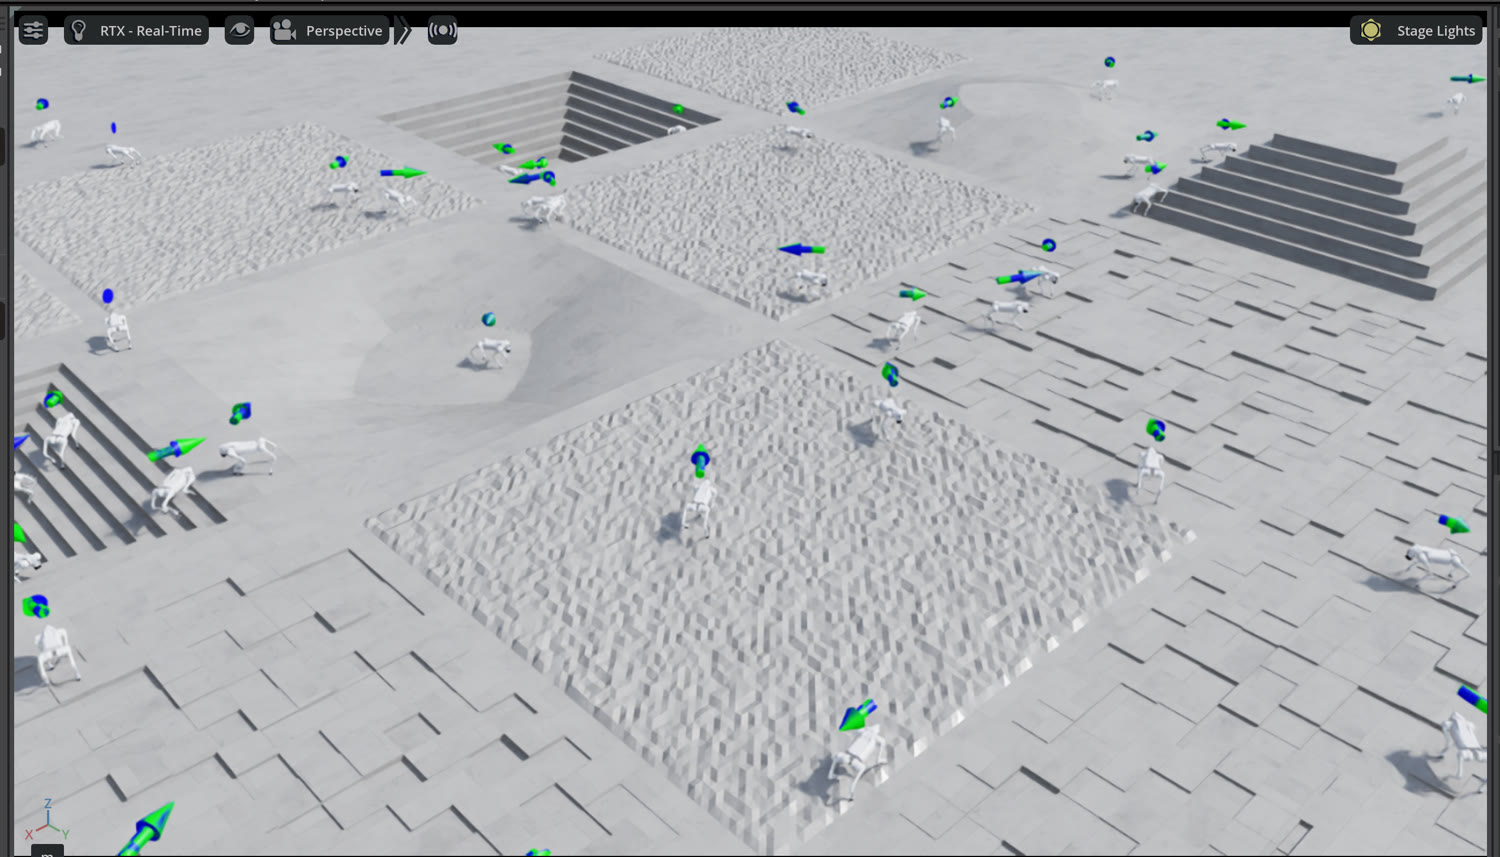
\includegraphics[width=0.485\textwidth]{figures/sim_rough.jpg}
\caption{Training in Isaac Lab with 16{,}384 parallel Go2 robots (arrows show each robot's
commanded velocity). Left: flat terrain, deployed zero-shot on the real robot. Right:
rough terrain with stairs and uneven blocks, validated in simulation; hardware deployment is
pending.}
\label{fig:terrain}
\end{figure*}

\subsection{Deployment}
The trained policy is exported to ONNX (452~KB) and TorchScript. A verified permutation
($\texttt{SIM\_TO\_REAL}=[3,0,9,6,4,1,10,7,5,2,11,8]$) reconciles the Isaac Lab joint order (PhysX
BFS) with the Unitree per-leg order. On the robot, a 50~Hz loop reads the IMU and encoders, builds
the 45-dim observation (the base linear velocity is not needed; it is critic-only), runs ONNX
inference ($\sim$1~ms), and sends joint targets to the 500~Hz driver PD loop; the built-in sport
mode is released first so it does not override low-level control. The same policy was run both
from a laptop over Ethernet and from the onboard Jetson Orin~NX, with consistent behaviour; the
Jetson allows fully untethered operation.

\section{Cognitive Approach}
\label{sec:cog}

The COGAR course frames every robot architecture on the same \textbf{Sense $\rightarrow$
Reasoning/Plan $\rightarrow$ Act} loop and distinguishes four families: \emph{hierarchical}
(Sense-Plan-Act, all three stages in sequence), \emph{reactive} (the Reasoning/Plan stage
removed), \emph{behaviour-based} (parallel sense-act behaviours with an arbitration step), and
\emph{hybrid reactive-deliberative}, also called cognitive (a direct Sense$\leftrightarrow$Act
loop with Reasoning/Plan on top). This section places the project on that map using the course's
own vocabulary, and connects the implementation to the course's design patterns and to Marr's
three levels of analysis.

\subsection{The project is a reactive architecture}
At run time the locomotion policy is a tight \textbf{Sense $\rightarrow$ Act} loop with the
\emph{Reasoning/Plan stage removed} (Fig.~\ref{fig:loop}): it senses (IMU and encoders), maps the
observation directly to motor targets, and never plans or maintains a world model. In the course
taxonomy this is exactly the \emph{reactive} family. The course defines a \textbf{behaviour} as
``a mapping of sensory inputs to a pattern of motor actions used to achieve a task,'' decomposed
into a \emph{perceptual schema} and a \emph{motor schema}; the policy is precisely such a
behaviour, with the observation construction as its perceptual schema and the joint-offset output
(through the PD loop) as its motor schema. The course's System\,1/System\,2 reading also fits:
the policy is a \emph{Type-1, reactive} behaviour that has been ``compiled down'' from a slow
optimisation, which is what reinforcement learning literally does, turning deliberative credit
assignment at training time into a fast model-free reaction at run time.

\begin{figure}[t]
\centering
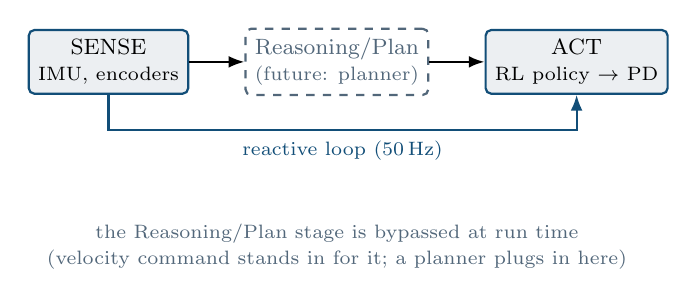
\begin{tikzpicture}[font=\footnotesize,
  st/.style={rounded corners=2pt, draw=accent, line width=0.8pt, fill=soft,
             minimum width=1.9cm, minimum height=0.8cm, align=center},
  pl/.style={rounded corners=2pt, draw=steel, dashed, line width=0.8pt,
             minimum width=1.9cm, minimum height=0.8cm, align=center, text=steel},
  ar/.style={-{Latex[length=2mm]}, line width=0.8pt}]
\node[st] (sense) {SENSE\\\scriptsize IMU, encoders};
\node[pl, right=0.7cm of sense] (plan) {Reasoning/Plan\\\scriptsize (future: planner)};
\node[st, right=0.7cm of plan] (act) {ACT\\\scriptsize RL policy $\to$ PD};
\draw[ar] (sense) -- (plan);
\draw[ar] (plan) -- (act);
\draw[ar, accent] (sense.south) -- ++(0,-0.45) -| node[pos=0.25,below]{\scriptsize reactive loop (50\,Hz)} (act.south);
\node[align=center, below=1.5cm of plan, text=steel] {\scriptsize the Reasoning/Plan stage is bypassed at run time\\\scriptsize (velocity command stands in for it; a planner plugs in here)};
\end{tikzpicture}
\caption{The deployed controller on the course's Sense-Reasoning/Plan-Act loop. The
Reasoning/Plan stage is removed (dashed): the system is a \emph{reactive} architecture, with the
velocity command as the interface where a deliberative layer would later attach.}
\label{fig:loop}
\end{figure}

\subsection{Behaviour coordination and subsumption}
A single reactive behaviour is not enough on hardware: something must decide \emph{when} it runs
and stop it before it breaks the robot. The deployment finite-state machine
$\textsc{idle}\to\textsc{stand\_up}\to\textsc{ready}\to\textsc{walk}\to\textsc{damping}\to
\textsc{stopped}$ provides this, and it is a textbook instance of the course's \textbf{behaviour
coordination}. It is \emph{competitive}, winner-take-all coordination by \emph{fixed priority}: a
small set of safety reflexes (a tilt reflex above $46^\circ$, a 100~ms sensor watchdog, a NaN/Inf
guard, action and joint clipping) sit above the walking behaviour and, when triggered,
\emph{suppress} it, in the precise sense of Brooks' subsumption taught in the course, where
suppression replaces the signal a behaviour sends to the actuators. These reflexes are also
``reflexes'' in the ethological sense the course gives: rapid, automatic, involuntary responses
correlated with stimulus strength, the kind the course notes are ``used for locomotion.'' The
system therefore realises the lower part of a behaviour-based architecture: a learned reactive
skill, coordinated and protected by a fixed-priority arbiter.

\subsection{Realising the course's design patterns}
The deployment code is built from the software design patterns the course teaches for robot
architectures. The sensing path is the \textbf{Sensor-device} pattern (the IMU and encoder
readers are pure, periodic data producers wrapping the SDK driver) feeding a
\textbf{Publish-subscribe} channel (the Unitree DDS / ROS\,2 topics push state to the controller,
which never assumes who is listening). The policy step is the \textbf{Computational} pattern: one
periodic \texttt{on\_update()} that collects all input ports (the observation), runs a single
inference, and publishes all outputs (the joint targets), with no blocking calls in the loop.
Most directly, the joint-order remapping is the \textbf{Adapter} pattern in its textbook form,
translating between two index conventions (Isaac Lab BFS and the Unitree per-leg order) exactly as
the course's Adapter example translates between coordinate systems.

\subsection{Marr's levels and the reference architecture}
The course uses Marr's three levels as the bridge from biology to software. Read that way, the
project is: \emph{Level~1 (what)}, a quadruped should walk and recover, an existence proof from
ethology; \emph{Level~2 (how, as processes)}, the perceptual and motor schemas of the policy
behaviour plus the fixed-priority coordinator (a finite-state machine); and \emph{Level~3
(implementation)}, ONNX inference on the Jetson with a PD loop on the motor driver. Within the
course's reference cognitive architecture (Darvish et al.~\cite{darvish2021}), which maps
Task~Representation/Manager and the Knowledge~Base to Reasoning/Plan and the Execution Manager,
Path~Planner and Controller to Act, this project implements the \textbf{Act / Controller} role:
the reusable locomotion competence on which a future Reasoning/Plan layer (a navigation or task
planner issuing velocity commands, the hybrid reactive-deliberative family) would stand. Task and
motion planning, which the course raises in the hierarchical lecture, is the natural way to close
that loop.

\section{Results and Congruence}
\label{sec:results}

\subsection{Simulation validation and the two-config comparison}
Both configurations were replayed in Isaac Sim across command directions, the stand-still command
and perturbations (pushes, friction changes, added payload). The best flat policy reaches the
metrics in Table~\ref{tab:metrics}: a 99.7\% survival rate, a 0.22~m/s velocity-tracking error,
and a final return of about 31.2. In simulation the two configurations are nearly
indistinguishable, which confirms \textbf{H1}: the gap is invisible in simulation, so a
simulation-only study would not reveal it.

\begin{table}[t]
\caption{Simulation metrics (best flat policy).}
\label{tab:metrics}
\centering
\footnotesize
\begin{tabular}{l r}
\toprule
\textbf{Metric} & \textbf{Value} \\
\midrule
Episode survival rate & \textbf{99.7\%} \\
Fall rate (base contact) & 0.33\% \\
Velocity tracking error & \textbf{0.22~m/s} \\
Angular velocity tracking error & 0.15~rad/s \\
Final mean return & ${\approx}31.2$ \\
\bottomrule
\end{tabular}
\end{table}

\subsection{Real-robot deployment}
On the physical Go2 EDU the same network that finished training runs unchanged at 50~Hz
(Fig.~\ref{fig:real}). Config~A drifts sideways; Config~B walks straight, confirming \textbf{H2}:
the asymmetric actor-critic, by keeping the policy inside its own perceptual horizon, removes the
drift. The heavier action-rate penalty and the latency randomization remove the motor chatter,
confirming \textbf{H3}. With a neutral command the policy holds station rather than trotting in
place, the effect of stand-still training. The rough-terrain policy is validated in simulation,
including stair climbing, but is not yet deployed on hardware, because the Go2 used has no depth
sensor feeding the height-scan observation.

\begin{figure}[t]
\centering
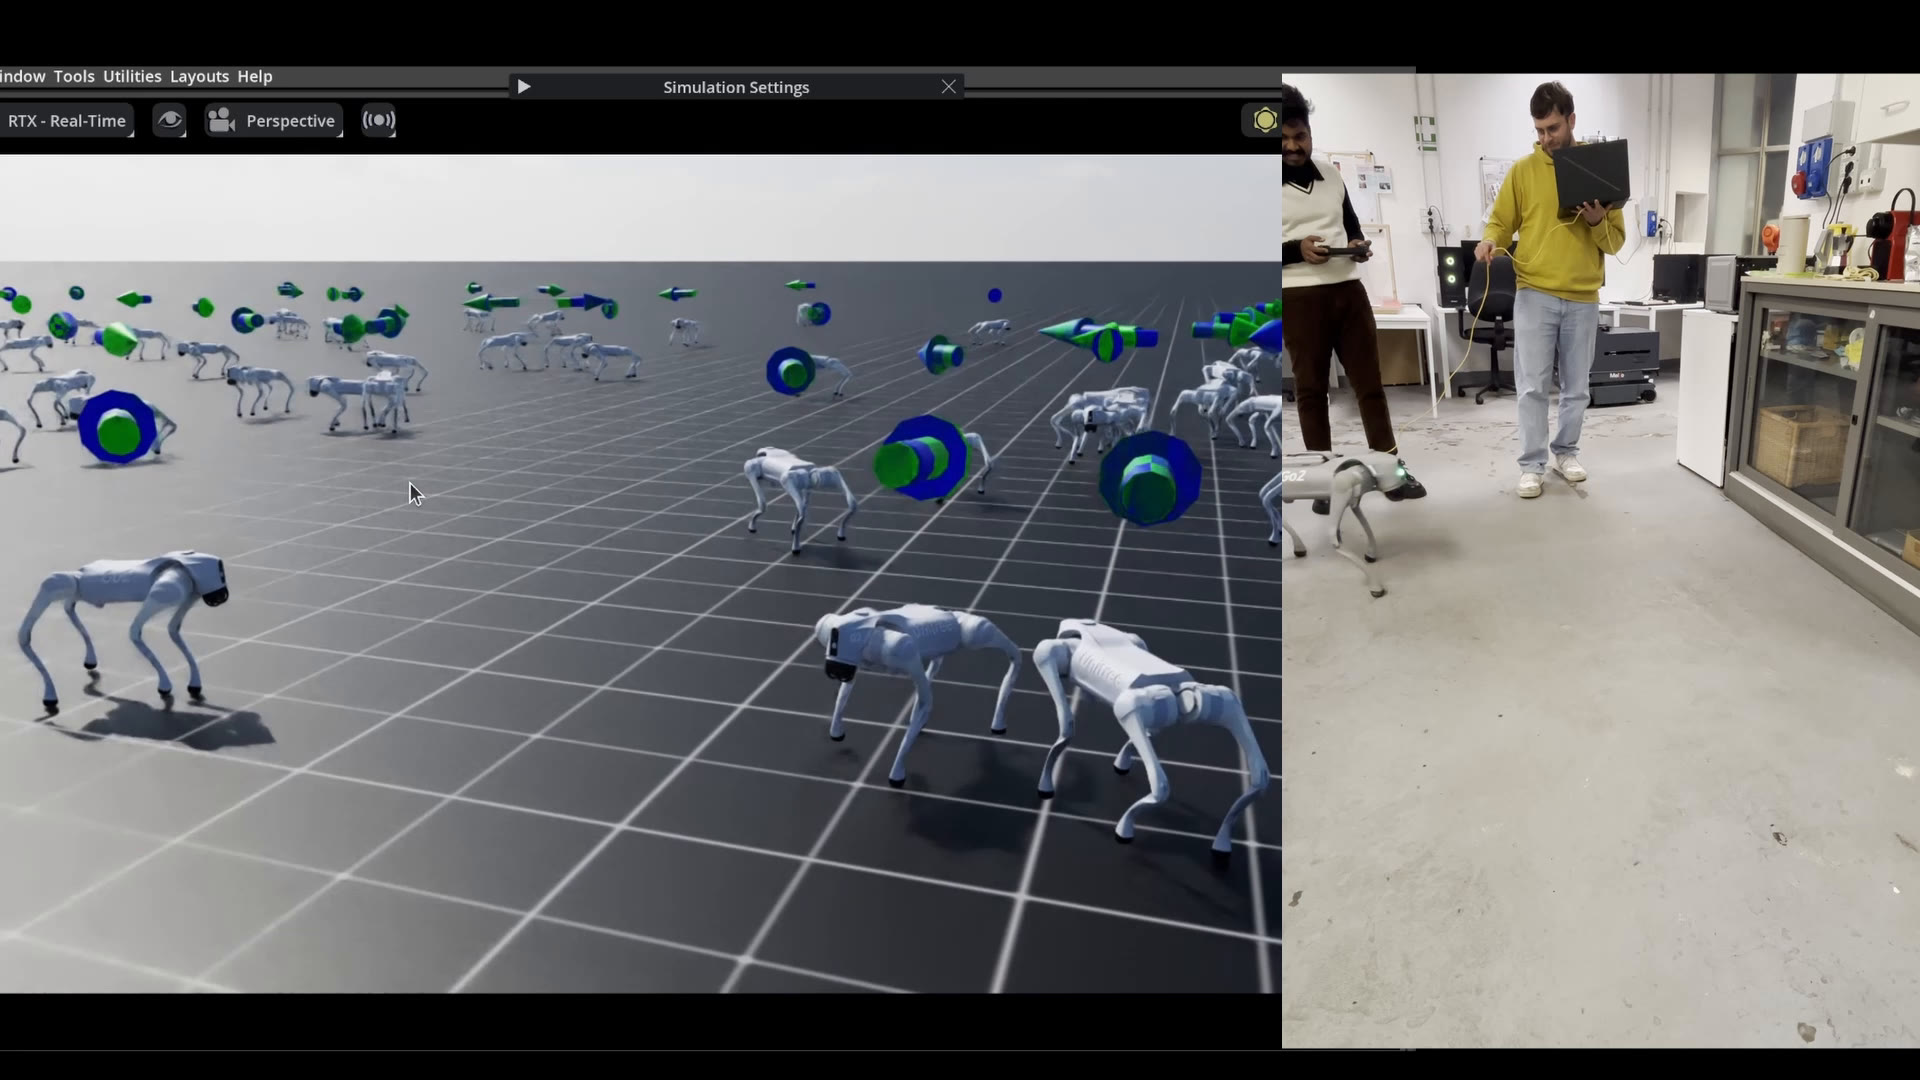
\includegraphics[width=0.96\columnwidth]{figures/real_deploy.jpg}
\caption{Zero-shot deployment. Left: Isaac Sim validation. Right: the real Unitree Go2 EDU
walking under joystick command, running the same ONNX policy that finished training.}
\label{fig:real}
\end{figure}

\subsection{Sim-to-real gap analysis}
The final policy is the result of fixing a sequence of failures, each exposing one mismatch
(Table~\ref{tab:gap}); the version history V1$\to$V2$\to$V3 records the process. The largest
single improvement was the asymmetric actor-critic (failure four).

\begin{table}[t]
\caption{Sim-to-real failures and fixes.}
\label{tab:gap}
\centering
\footnotesize
\begin{tabular}{p{1.5cm} p{2.5cm} p{2.6cm}}
\toprule
\textbf{Failure} & \textbf{Root cause} & \textbf{Fix} \\
\midrule
Foot dragging & air-time reward too low & $\times40$ air-time, feet-slide penalty \\
Collapsing & orientation penalty too harsh & rebalance: tracking dominates \\
Motor chatter & actions change too fast & $\times5$ action-rate, accel.\ penalty \\
\textbf{Sideways drift} & actor used base velocity it cannot measure & \textbf{asymmetric actor-critic} \\
Gain sensitivity & real latency, gains, stiction & \texttt{DelayedPDActuator}, $\pm20\%$ gains \\
Twisted motion & sim vs SDK joint order & verified joint remap (Adapter) \\
\bottomrule
\end{tabular}
\end{table}

\subsection{Congruence of results and conclusions}
We keep the claims conservative. \emph{Zero-shot flat walking on the real Go2} is supported by the
demonstration and by the disappearance of the specific failure modes. \emph{The asymmetric
actor-critic removes drift} is supported by the V2-versus-V3 comparison (H2). \emph{Domain
randomization bridges the gap} is supported by robustness across the training distribution. The
honest scope is also stated: the simulation metrics are quantitative, whereas the hardware
comparison is qualitative, and a logged real-robot benchmark (cost of transport, measured
tracking, push recovery) remains future work; the rough-terrain policy is validated only in
simulation; and, in cognitive-architecture terms, the project realises the reactive behaviour and
its fixed-priority coordinator, not a deliberative Reasoning/Plan layer. Adding that layer, a
planner issuing the velocity commands the policy already consumes, would complete the hybrid
reactive-deliberative architecture and is the clear next step, together with a depth sensor for
on-hardware rough-terrain locomotion and a learned estimator for the base velocity.

\section*{Acknowledgments}
The author thanks Prof.\ Fulvio Mastrogiovanni and Gianluca Galvagni for the Cognitive
Architectures for Robotics course and for their guidance and support throughout this project.

\begin{thebibliography}{99}
\footnotesize
\bibitem{rudin2022} N. Rudin et al., ``Learning to walk in minutes using massively parallel deep
RL,'' \emph{CoRL}, 2022.
\bibitem{schulman2017} J. Schulman et al., ``Proximal policy optimization algorithms,''
\emph{arXiv:1707.06347}, 2017.
\bibitem{tan2018} J. Tan et al., ``Sim-to-real: Learning agile locomotion for quadruped robots,''
\emph{RSS}, 2018.
\bibitem{hwangbo2019} J. Hwangbo et al., ``Learning agile and dynamic motor skills for legged
robots,'' \emph{Science Robotics}, vol.~4, no.~26, 2019.
\bibitem{tobin2017} J. Tobin et al., ``Domain randomization for transferring deep neural networks
from simulation to the real world,'' \emph{IROS}, 2017.
\bibitem{peng2018} X. B. Peng et al., ``Sim-to-real transfer of robotic control with dynamics
randomization,'' \emph{ICRA}, 2018.
\bibitem{pinto2018} L. Pinto et al., ``Asymmetric actor critic for image-based robot learning,''
\emph{RSS}, 2018.
\bibitem{lee2020} J. Lee et al., ``Learning quadrupedal locomotion over challenging terrain,''
\emph{Science Robotics}, vol.~5, no.~47, 2020.
\bibitem{miki2022} T. Miki et al., ``Learning robust perceptive locomotion for quadrupedal robots
in the wild,'' \emph{Science Robotics}, vol.~7, no.~62, 2022.
\bibitem{brooks1986} R. A. Brooks, ``A robust layered control system for a mobile robot,''
\emph{IEEE J. Robotics and Automation}, vol.~2, no.~1, 1986.
\bibitem{darvish2021} K. Darvish et al., ``A hierarchical architecture for human-robot cooperation
processes,'' \emph{IEEE Trans. Robotics}, vol.~37, no.~2, 2021.
\bibitem{marr1982} D. Marr, \emph{Vision}. W. H. Freeman, 1982.
\end{thebibliography}

\end{document}
